\begin{figure}[htp]
  \centering
  \begin{tikzpicture}
    \begin{axis}[width=0.98\textwidth, height=6cm, ylabel=Wellenlänge $\lambda$ in \si{\nano\metre}, xlabel=Radeinstellung in a.u., legend cell align={left}]
        \addplot[blue, thick] table[x index=0,y index=1, col sep=semicolon]{Daten/Eichung_SPM1_mitQuecksilberdapflampe.csv};
          \addplot[color=black,mark=*, only marks] coordinates {
    		(3.443, 2325)
    		(3.557, 1699.5)
        (3.635, 1529.5)
        (3.69, 1362)
        (3.783, 1128.6)
        (3.839, 1014)
        (4.328, 579)
        (4.412, 546.1)
    	};
      \legend{Exponentieller Fit, Messdaten};
      \node[anchor=west] (A) at (4.1,1400){\begin{tabular}{|c | c|}
        \hline
        Fit & $\exp(a+bx+cx^2)$\\
        \hline
        $a$ & $27.75\pm 0.70$ \\
        $b$ & $-9.17\pm 0.37$\\
        $c$ & $0.977 \pm 0.048$\\
        \hline
      \end{tabular}};
    \end{axis}
  \end{tikzpicture}
  \caption{Eichung der Prismenverstellung.}
  \label{fig:EichungSPM1}
\end{figure}

% \begin{figure}[htp]
%     \centering
%         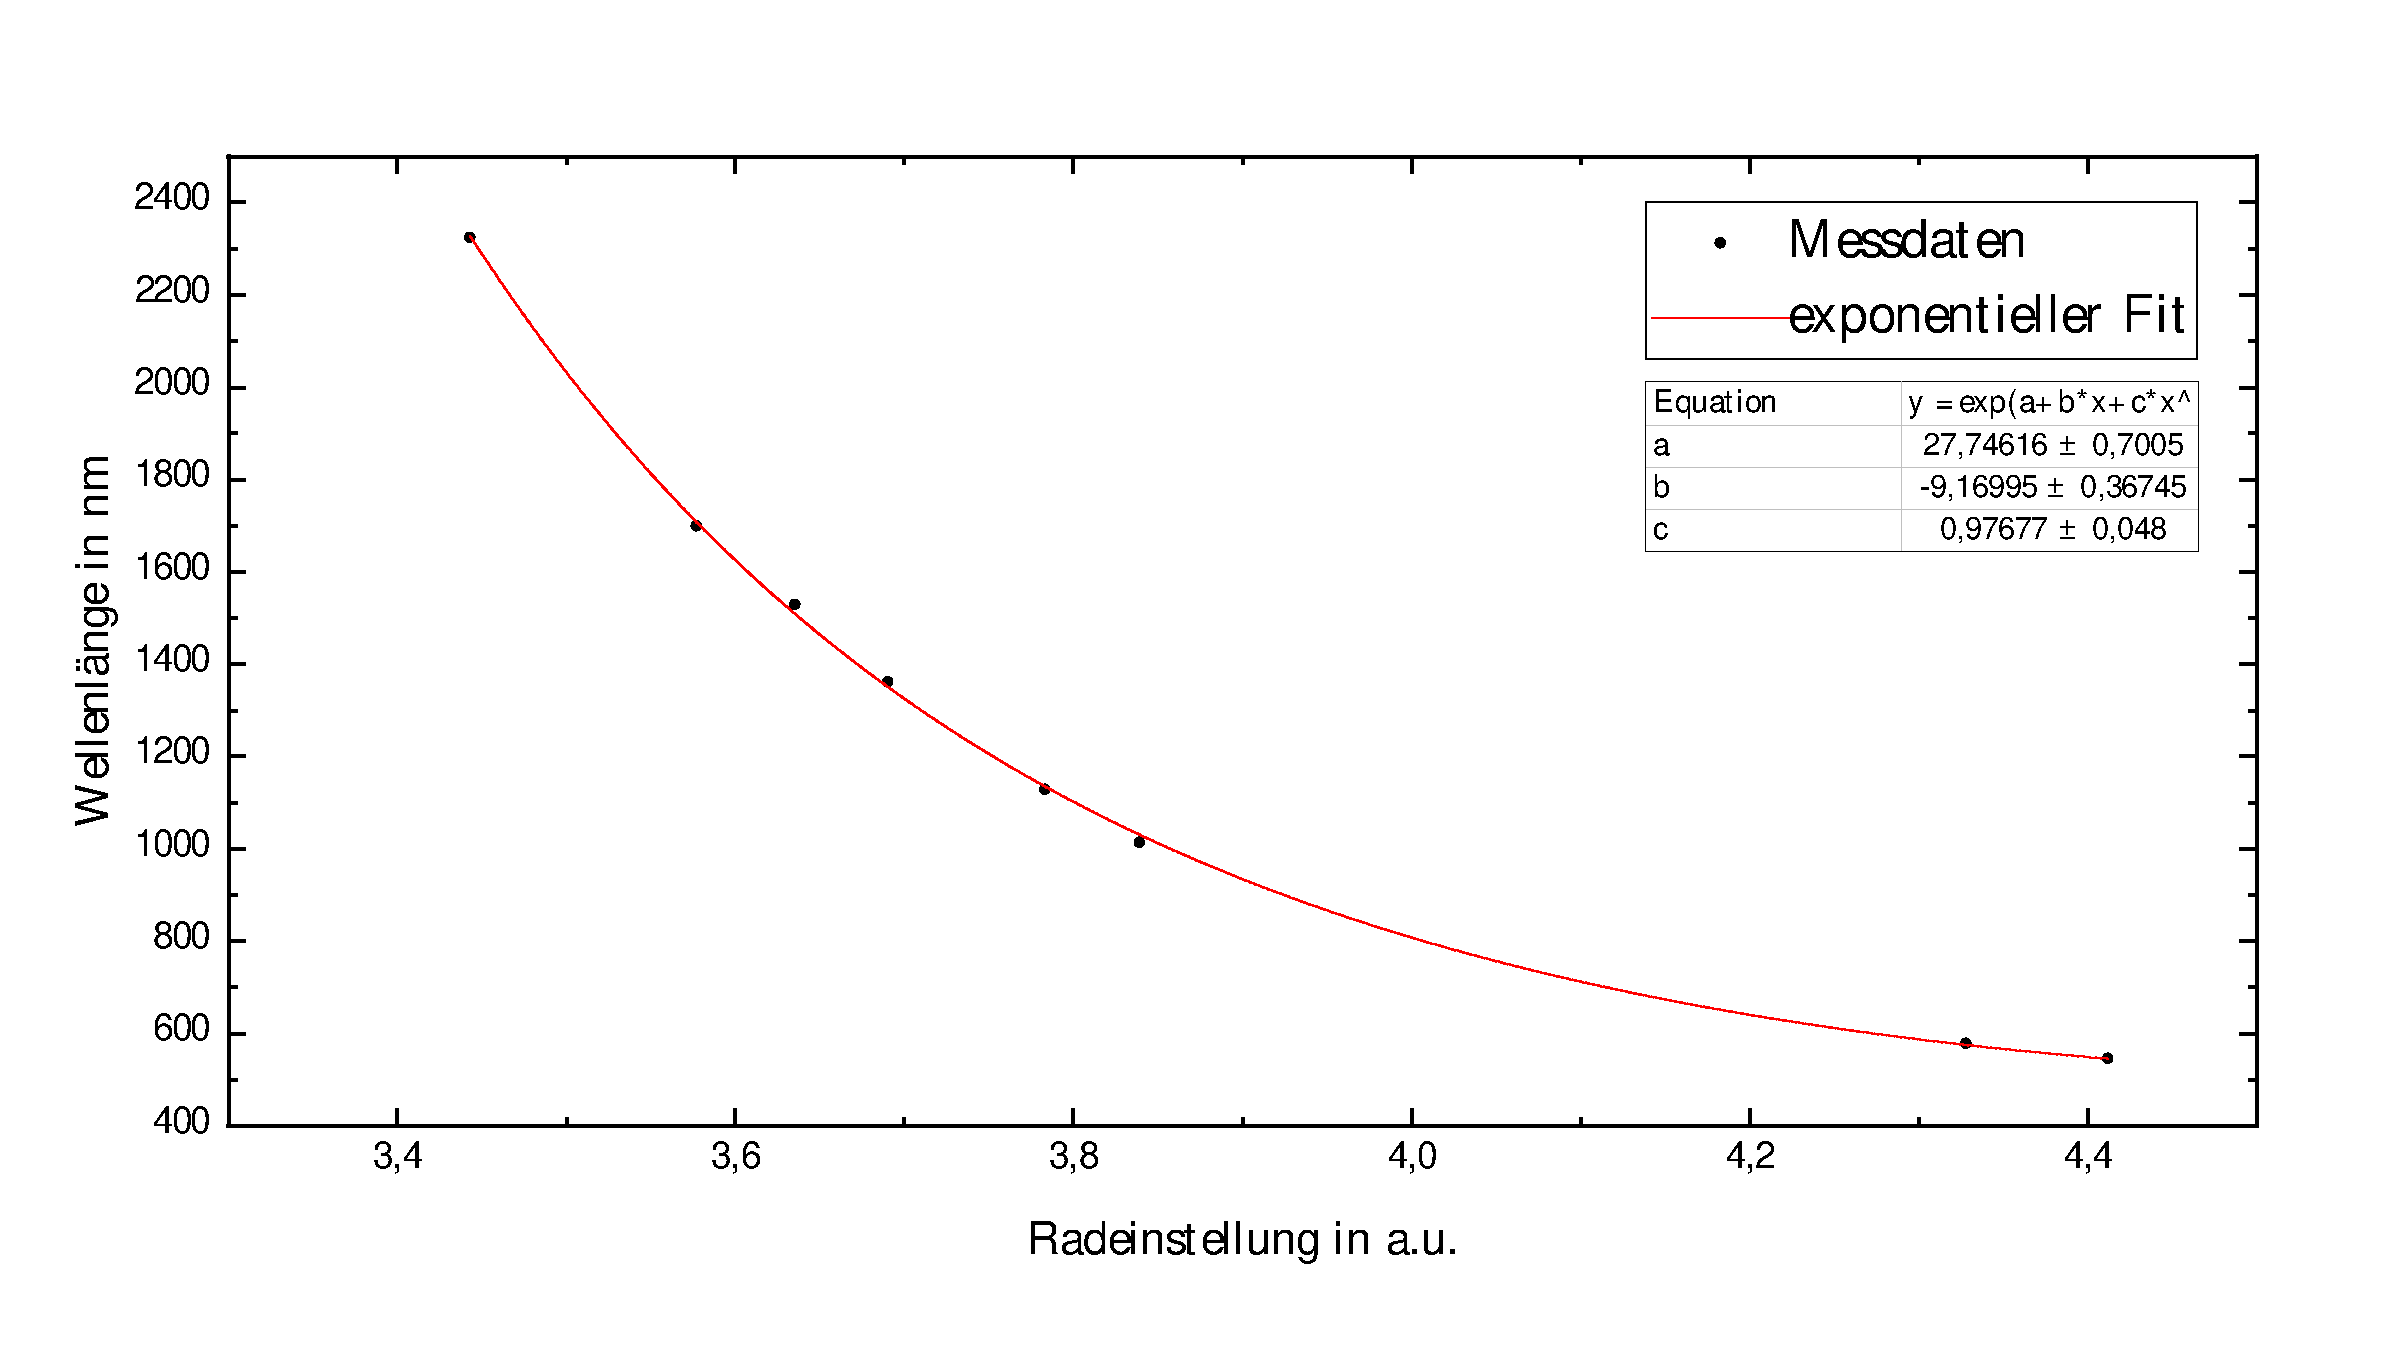
\includegraphics[width=0.9\textwidth]{Bilder/Eichung_SPM1_mitQuecksilberdapflampe.pdf}
%     \caption{Eichung der Prismenverstellung}
%     \label{fig:EichungSPM1}
% \end{figure}
